\section{Simulación}
\label{simulacion}

Para testar el funcionamiento del algoritmo se han realizado diferentes experimentos sobre el entorno de simulación robótica V-REP [ javi ]. V-REP es un simulador muy versátil que permite diferentes opciones a la hora de integrarse en un proyecto. Por un lado, está basado en el lenguaje Lua y ofrece un interprete integrado en el propio simulador, sin embargo, también permite utilizar programas externos en diversos lenguajes de programación como son: C++, Python o Java. Además, V-REP está integrado en ROS [ javi ] y pone a disposición del usuario los paquetes necesarios para realizar simulaciones de proyectos basados en ROS. En el caso que nos ocupa, se ha utilizado el lenguaje Python a través de la API proporcionada por V-REP para el control remoto de la simulación.

\subsection{Robot seleccionado}

Como base para implementar los algoritmos, se ha seleccionado un robot móvil con dos grados de libertad y configuración holonómica. V-REP contiene varios modelos de robots reales de este tipo, tales como: el javi , javi o el Pioneer 3D-X. Se ha utilizado este último, mostrado en la figura \ref{fig:pioneer}, dado que es un robot bastante usado en tareas de navegación, y su relación entre tamaño y prestaciones es adecuada para nuestro problema.

\begin{figure}[h]
		\centering
        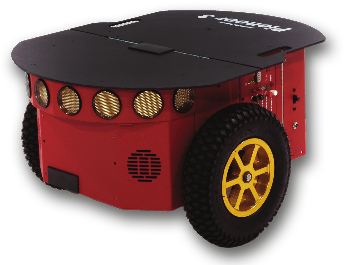
\includegraphics[width=0.5\textwidth]{images/pioneer.png}
        \caption{Robot Pioneer 3D-X}
        \label{fig:pioneer}
\end{figure} 

El Pionner 3D-X es un robot móvil impulsado por dos ruedas de movimiento diferencial. Junto a sus motores equipa encoders incrementales de 500 posiciones. También incluye sensores ultrasonicos de posición. Sin esta aplicación no ha sido necesario utilizar ningún sensor interno del robot. El Pionner 3D-X tiene unas dimensiones de 38.1x45.5x23.7 cm . Su velocidad se acerca a los 1.6 metros por segundo y tiene una capacidad de carga de hasta 23 kg.

\subsection{Desarrollo del controlador del robot}

La API remota de V-REP proporciona acceso al control de los actuadores del robot. Tomando como base la modificacion de parámetros de bajo nivel de los actuadores (velocidad y sentido de giro), se ha desarrollado un controlador que permite al robot desplazarse entre dos puntos con un error menor a 10cm. Teniendo en cuenta el tamaño del robot, se considera que es una precisión muy razonable.

El primer controlador implementado ha sido la función de giro y orientación. En nuestra aplicación, es muy importante realizar giros controlados, ya que repercutirán con gran importancia en la suavidad de los movientos del robot, así como en el tiempo ocupado en realizar la prueba. Por una parte, se requiere conocer en todo momento la orientación del robot respecto al eje de coordenadas global del simulador. Al mismo tiempo, el controlador debe permitir modificar esta orientación con el objetivo de dirigir el robot correctamente hacia los puntos objetivos. A continuación, en la figura \ref{fig:flujogiro} se muestra un diagrama de estados en el que se define el modo de actuación del robot tras una orden de giro.

\begin{figure}[h]
		\centering
        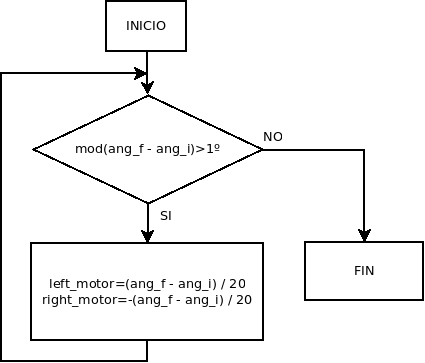
\includegraphics[width=0.5\textwidth]{images/flujogiro.png}
        \caption{Diagrama de estados del controlador de giros}
        \label{fig:flujogiro}
\end{figure} 

El segundo controlador del robot corresponde a su traslación. Ya que el robot constituye el punto de inicio de cualquier trayectoria que sea desarrollada, se debe conocer su posición inicial antes de correr el algoritmo de planificación. También, durante la simulación, se requiere un conocimiento en tiempo real de la posición global del robot. Este controlador nos permitirá definir el desplazamien y la consecución de objetivos del robot. En el siguiente diagrama de estados, representado en la figura \ref{fig:flujoavance}, se muestra la implementación de este controlador.

\begin{figure}[h]
		\centering
        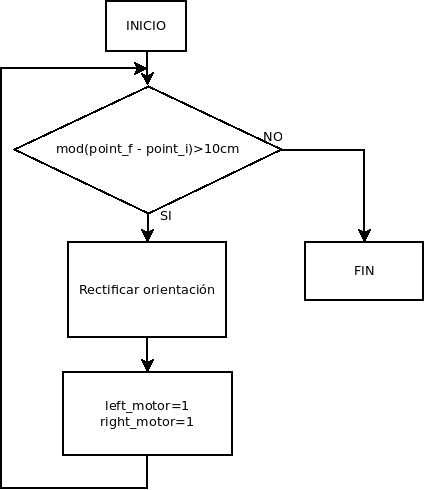
\includegraphics[width=0.5\textwidth]{images/flujoavance.png}
        \caption{Diagrama de estados del controlador de desplazamiento}
        \label{fig:flujoavance}
\end{figure} 

\subsection{Escenarios de simulación}

Los escenarios propuestos se han diseñado para probar la eficacia del algoritmo frente a diferentes situaciones problemáticas. Entre los puntos críticos de los escenarios destacan: tuneles con una altura definida, pasillos estrechos y zigzagueos. El uso de bloques sólidos modulares permite realizar configuraciones precisas para probar de forma directa las capacidades del algoritmo. Se han diseñado 3 escenarios con un area de javi m.

\begin{itemize}
	\item Escenario A: Túneles y obstáculos de diferente altura. Puede observarse en la figura \ref{fig:escenario1}.	
	
	
\begin{figure}[h]
		\centering
        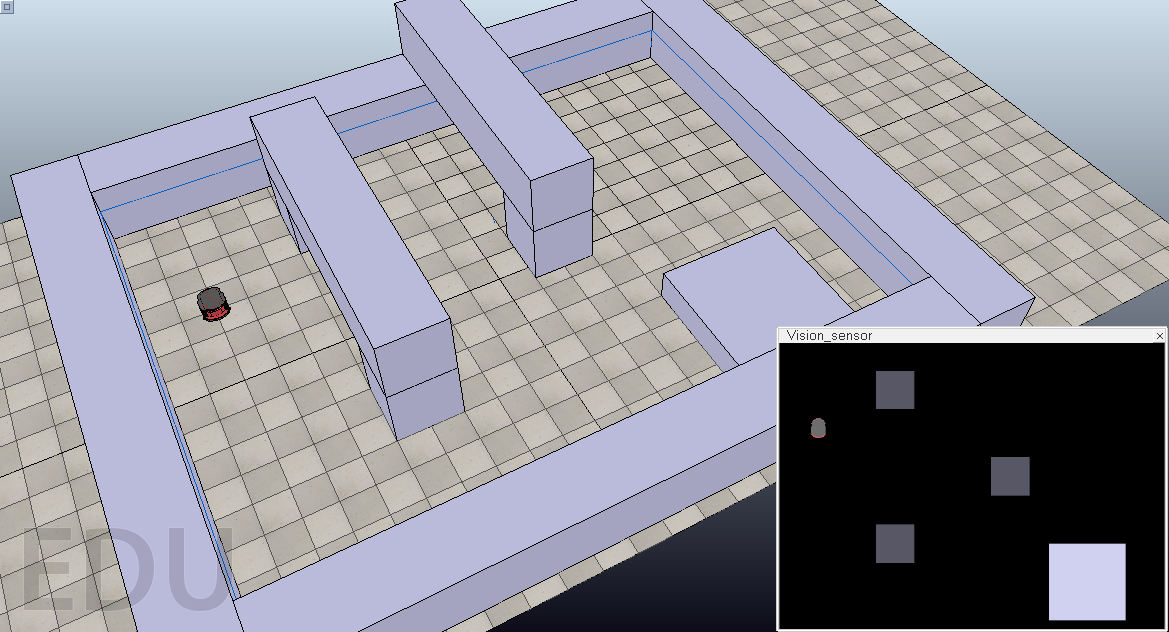
\includegraphics[width=0.7\textwidth]{images/escenario1}
        \caption{Escenario numero 1}
        \label{fig:escenario1}
\end{figure} 
	
	\item Escenario B: Zigzagueo constante y pasillos estrechos. Puede observarse en la figura \ref{fig:escenario2}.
	
		
\begin{figure}[h]
		\centering
        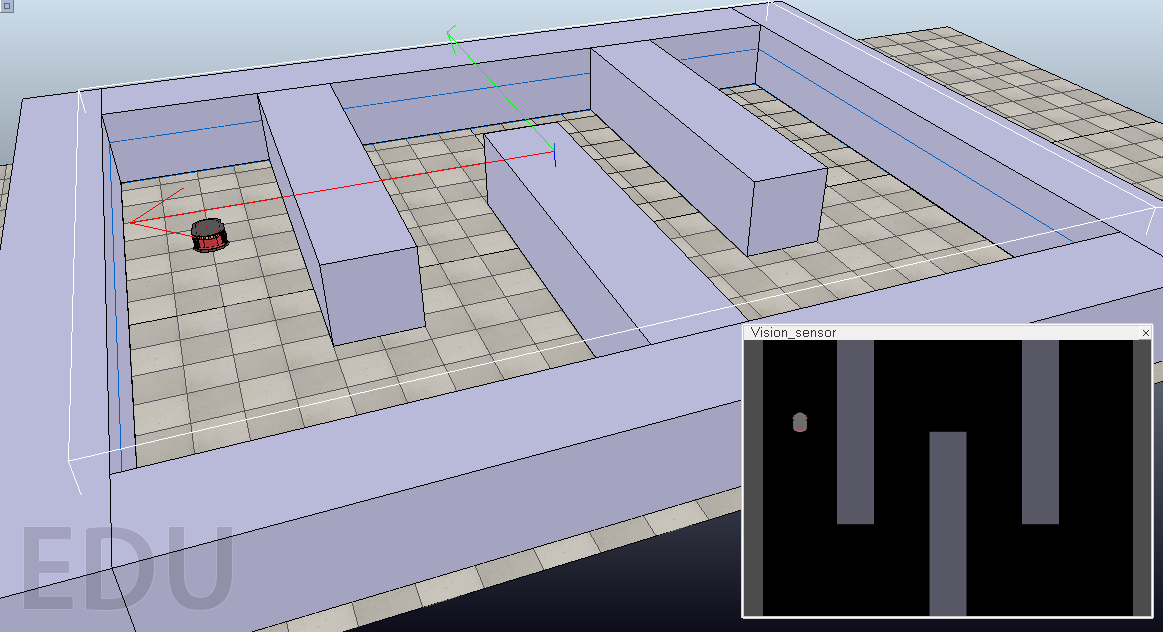
\includegraphics[width=0.7\textwidth]{images/escenario2.png}
        \caption{Escenario numero 2}
        \label{fig:escenario2}
\end{figure} 
	
	\item Escenario C: Integración de túneles, zigzagueos y pasillos estrechos. Puede observarse en la figura \ref{fig:escenario3}.

	
\begin{figure}[h]
		\centering
        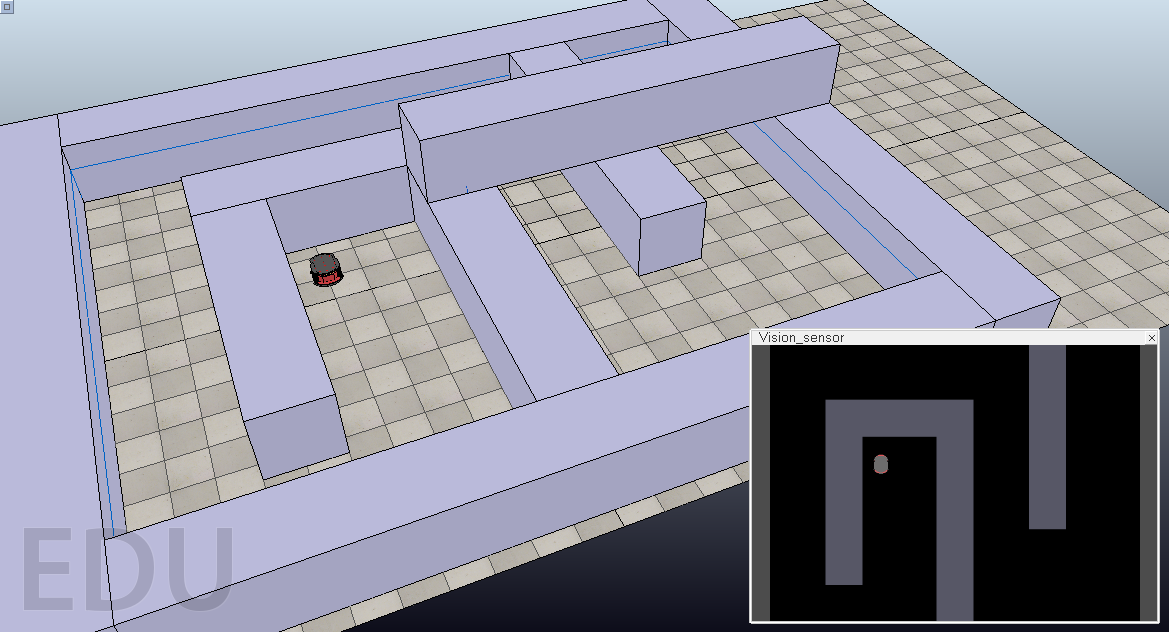
\includegraphics[width=0.7\textwidth]{images/escenario3.png}
        \caption{Escenario numero 3}
        \label{fig:escenario3}
\end{figure} 

\end{itemize}




\subsection{Extracción de datos del simulador}

Uno de los puntos mas interesantes al trabajar con V-REP es la generación de planos a partir de los escenarios. La aplicación desarrollada está programada para funcionar en dos dimensiones, sin embargo, para crear los mapas se han tenido en cuenta tres dimensiones. El motivo de esto es obtener un funcionamiento óptimo del robot en situaciones cuya cruzabilidad se vea comprometida. Los casos más numerosos son aquellos en los que el robot se enfrenta al paso bajo un obstáculo elevado. 

Para extraer el plano se ha utilizado una cámara aérea de proyección ortogonal. Su rango de visión abarca la superficie completa del escenario y está situada a una altura ligeramente superior a la del robot. Dicho de otra forma, la cámara captará todos los objetos que se encuentren en el escenario que intercedan en el volumen mínimo sobre el que puede garantizarse la cruzabilidad.

En las imágenes de la figura \ref{fig:tunel} se puede observar que los obstáculos cuya altura es superior al robot, no se tienen en cuenta a la hora de procesar el algoritmo.

	
\begin{figure}[h]
		\centering
        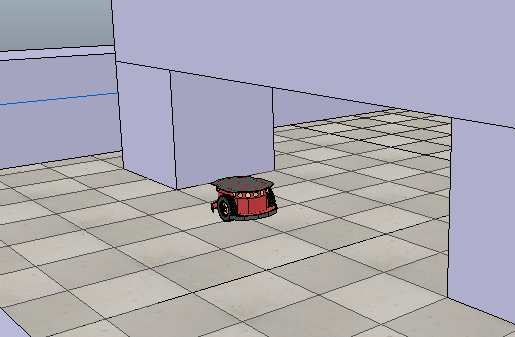
\includegraphics[width=0.7\textwidth]{images/tunel.png}
        \caption{Obstáculo elevado. La linea azul del fondo representa la altura mínima requerida para garantizar la cruzabilidad.}
        \label{fig:tunel}
\end{figure} 

Las imágenes son transferidas desde el simulador al programa principal, dónde se les aplica el algoritmo y comienza la ejecución.

